\chapter{TINJAUAN PUSTAKA}\label{tinjauan pustaka}


\section{Material dan Konstruksi \textit{Bundengan}}\label{subBab:konstruksiBundengan}
\Bundengan adalah alat musik yang unik dan luar biasa \cite{kunst}. Pasalnya, alat musik yang dimainkan dengan cara memetik senar-\textit{bandulan} ini dapat menghasilkan bunyi seperti layaknya alat musik logam, yaitu gamelan \cite{illusiveSound}. Selain itu, petikan pada bilah bambu juga menghasilkan bunyi layaknya kendang \cite{skripsiSaid}. Material dan konstruksi \bundengan sangat berpengaruh terhadap bunyi \bundengan yang unik ini.  \par 
Salah satu ciri musik tradisional adalah digunakannya peralatan yang sangat sederhana \cite{bukuMusik}. Hal ini juga berlaku pada \textit{bundengan}. Material penyusun alat musik ini dapat dengan mudah ditemukan di lingkungan sekitar wilayah Wonosobo, Jawa Tengah. Material penyusun tersebut berasal dari bambu, ijuk, dan senar badminton. Berdasarkan keterangan Yatno, salah seorang pengrajin \textit{bundengan}, material yang ia butuhkan didapatkan dari sekitar rumahnya yang mana masih banyak terdapat pohon bambu dan ijuk \cite{videoBundenganTNTF}.  \par 
Sebagian besar struktur \bundengan berasal dari bambu. Bagian dari pohon bambu yang digunakan di antaranya adalah potongan batang bambu (Gambar \ref{fig:potonganBambuMentah}), ranting bambu, dan pelepah buluh bambu atau \textit{slumpring} (Gambar \ref{fig:slumpring}). Jenis bambu yang dipilih adalah bambu apus, sebab bambu ini lebih elastis jika dibandingkan dengan bambu jenis lain \cite{skripsiSaid}. Potongan bambu dianyam membentuk struktur utama \textit{kowangan}, seperti yang diperlihatkan pada Gambar \ref{fig:menganyamKerangka}. Setelah dianyam, bagian ujung anyaman akan dirapatkan sehingga membentuk seperti \kowangan (Gambar \ref{fig:memincukKerangka}). Selain digunakan sebagai penyusun kerangka \textit{kowangan}, potongan bambu yang lebih kecil (Gambar \ref{fig:bilahBambuMentah}) juga dijadikan sebagai komponen penghasil bunyi kendang pada \textit{bundengan}, seperti yang sudah diperlihatkan pada Gambar \ref{fig:bilahBambu}. Ranting bambu adalah cabang batang bambu yang memiliki diameter lebih kecil \cite{skripsiSaid}. Potongan ranting bambu ini digunakan sebagai \textit{bandulan}, yaitu komponen yang menggantung pada senar \textit{bundengan}. Gambar \ref{fig:senarBandulan} memperlihatkan \textit{bandulan} yang berada di tengah-tengah senar \textit{bundengan}. Pelepah buluh bambu atau \textit{slumpring} merupakan jenis dedaunan yang tumbuh di bagian ruas batang bambu \cite{skripsiSaid}. \textit{Slumpring} digunakan sebagai pelapis anyaman bambu supaya dapat difungsikan sebagai tudung. \textit{Slumpring} dipilih karena bagian luarnya bersifat hidrofobik atau menolak air, sehingga tidak tembus oleh air hujan. Gambar \ref{fig:memasangSlumpring} memperlihatkan proses pemasangan \textit{slumpring} pada kerangka anyaman \textit{kowangan}. \par 
\begin{figure}[b!]
    \centering
    \subfigure[]{\label{fig:potonganBambuMentah}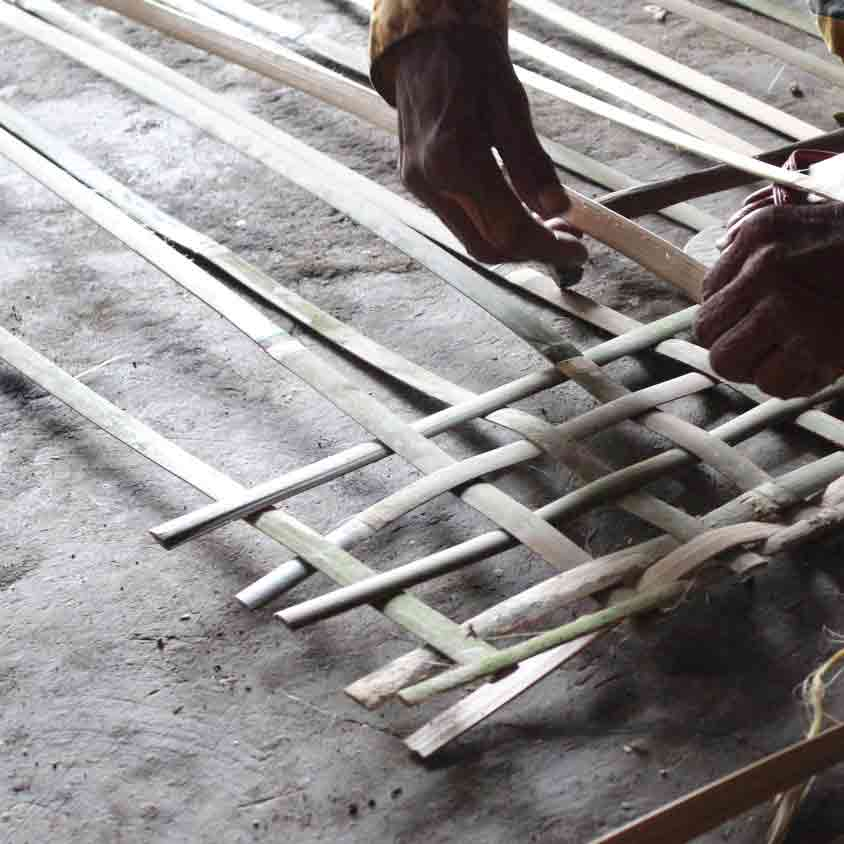
\includegraphics[width=47mm]{Gambar/potonganBambu.jpg}}
    \hspace{0.5cm}
    \subfigure[]{\label{fig:slumpring}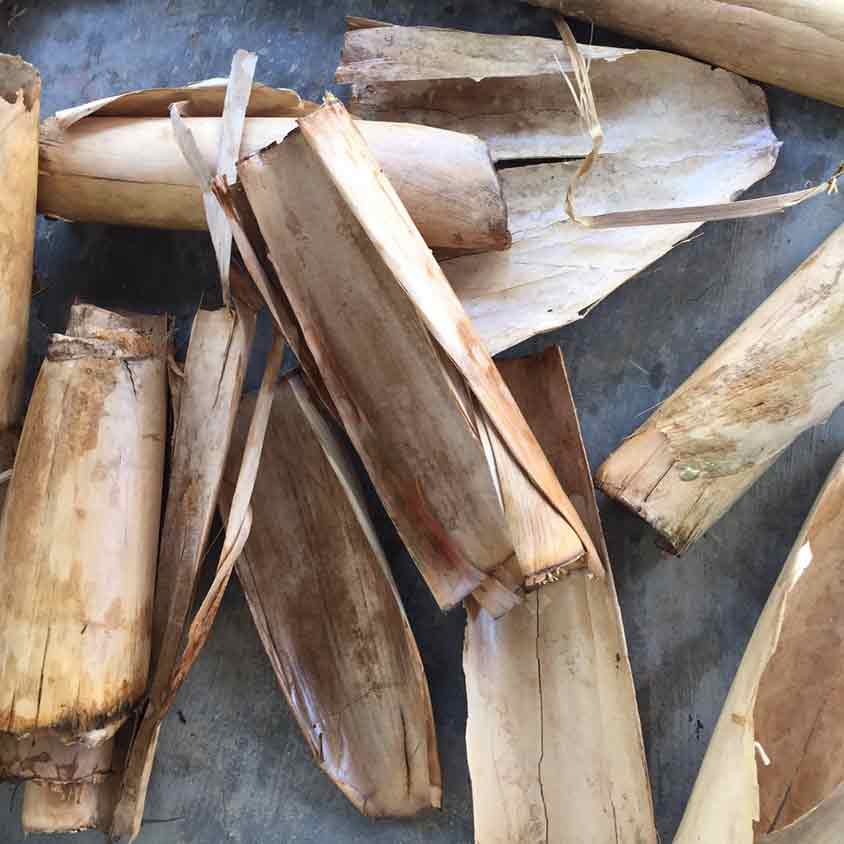
\includegraphics[width=47mm]{Gambar/slumpring.jpg}}
    \hspace{0.5cm}
    \subfigure[]{\label{fig:bilahBambuMentah}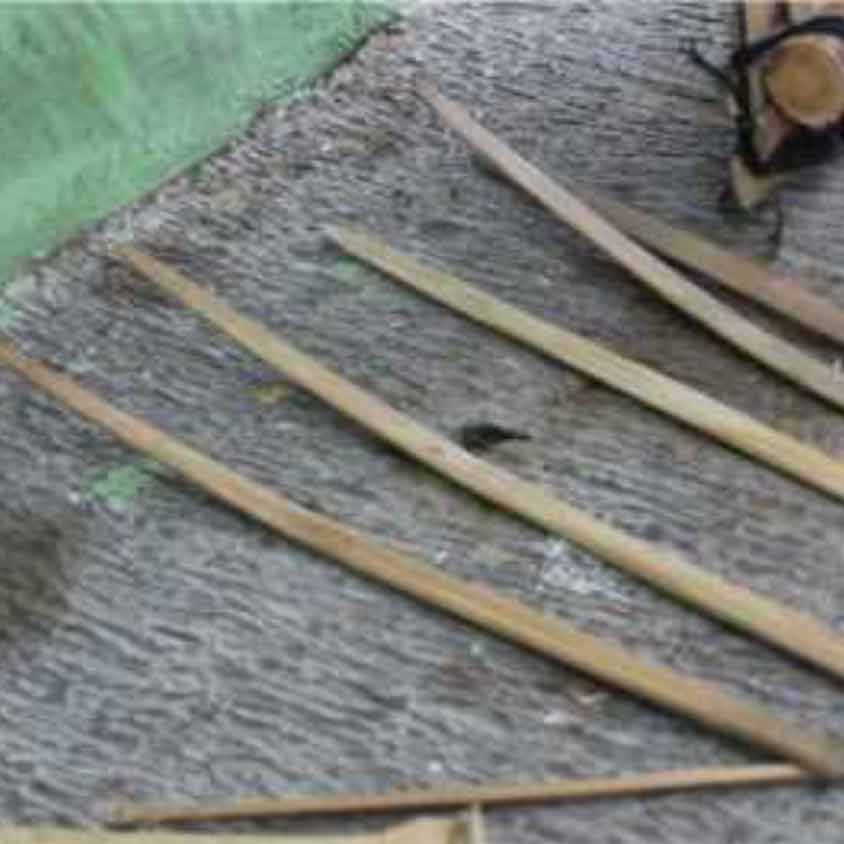
\includegraphics[width=47mm]{Gambar/bilahBambu-mentah.jpg}}
    \caption{Beberapa bagian bambu yang digunakan sebagai material penyusun \textit{bundengan}; (a) potongan bambu \cite{palmer}, (b) \textit{slumpring} \cite{videoBundenganTNTF}, dan (c) bilah bambu \cite{skripsiSaid}.}
    \label{fig:bagianBambu}
\end{figure}
\begin{figure}[t!]
    \centering
    \subfigure[]{\label{fig:menganyamKerangka}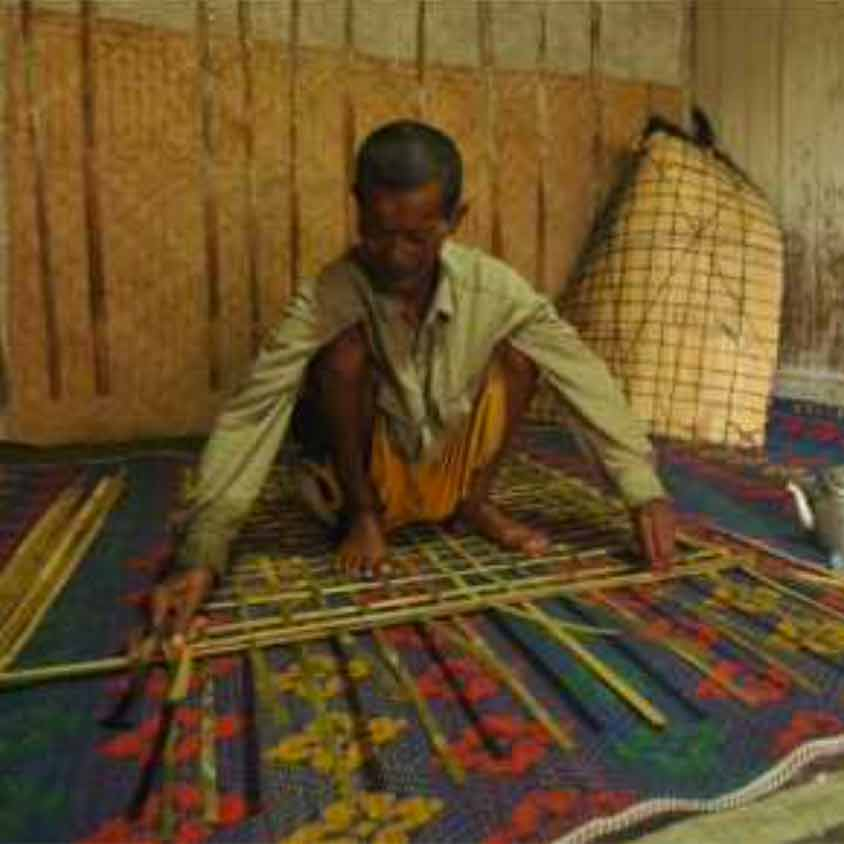
\includegraphics[width=47mm]{Gambar/menganyamKerangka.jpg}}
    \hspace{0.5cm}
    \subfigure[]{\label{fig:memincukKerangka}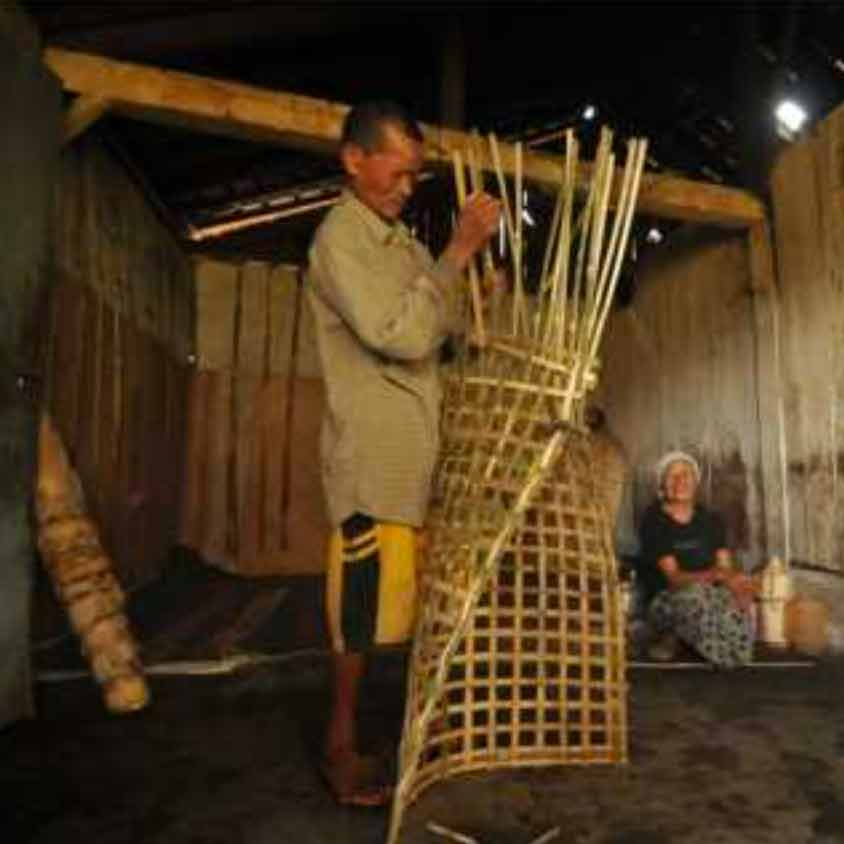
\includegraphics[width=47mm]{Gambar/memincukKerangka.jpg}}
    \hspace{0.5cm}
    \subfigure[]{\label{fig:memasangSlumpring}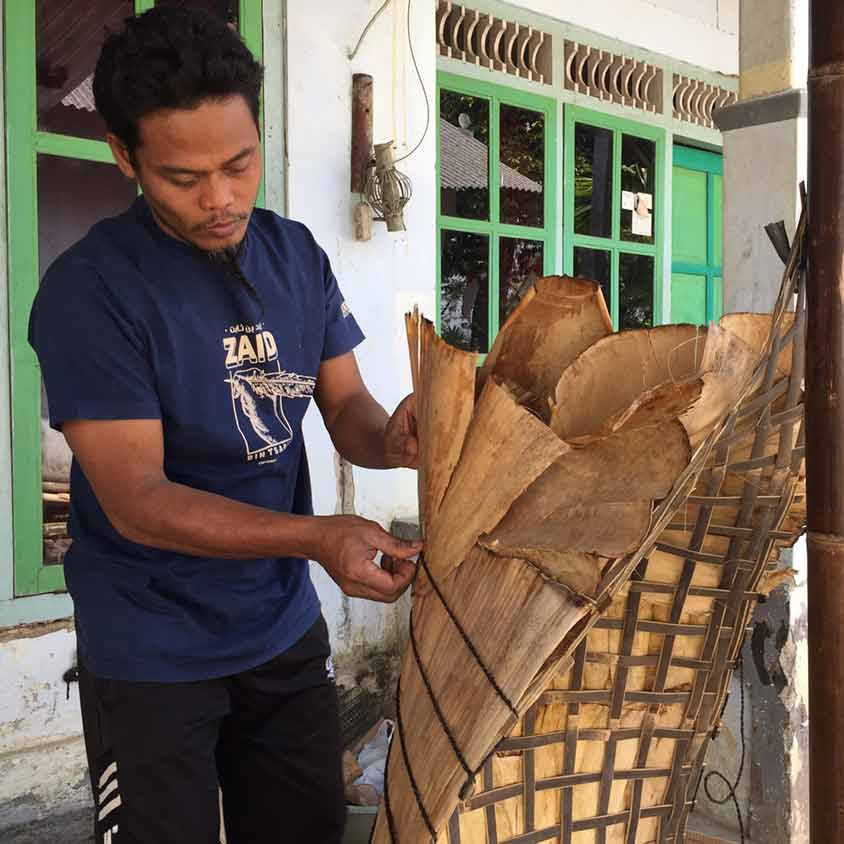
\includegraphics[width=47mm]{Gambar/memasangSlumpring.jpg}}
    \hspace{0.5cm}
    \subfigure[]{\label{fig:mengikatIjuk}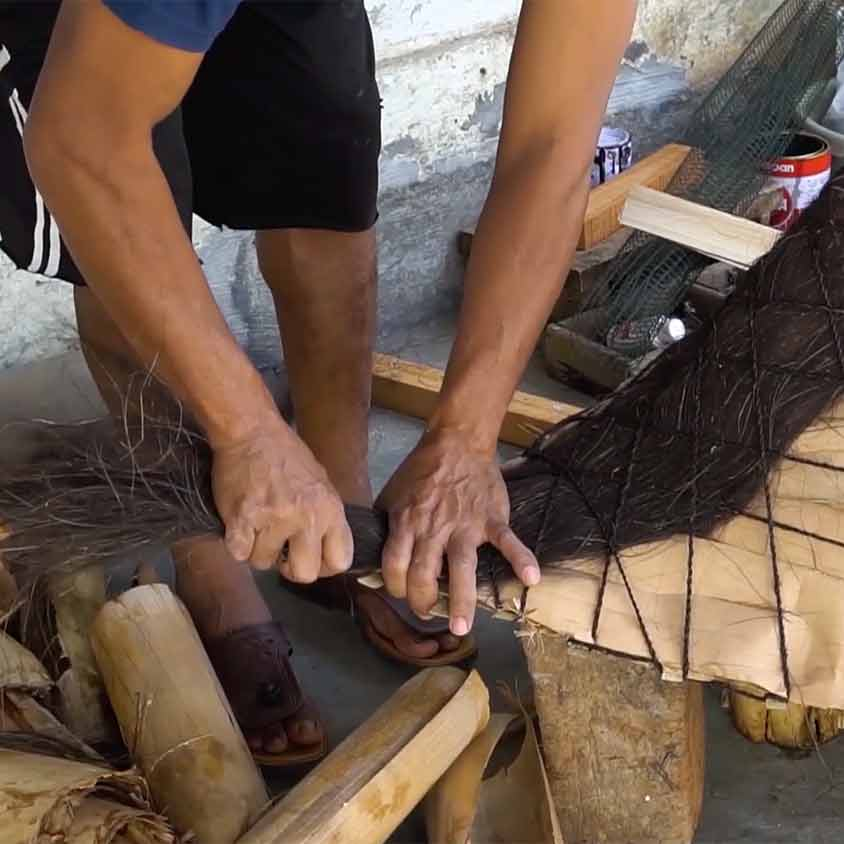
\includegraphics[width=47mm]{Gambar/mengikatIJUK.jpg}}
    \caption{Proses pembuatan \textit{kowangan}; Mahrumi sedang (a) menganyam kerangka kemudian (b) memincuk ujung kerangka \cite{skripsiSaid}, sedangkan Yatno (c) memasang \textit{slumpring} lalu (d) mengikatnya dengan ijuk \cite{videoBundenganTNTF}.}
    \label{fig:membuatKowangan}
\end{figure}
Selain bambu, bahan lain yang digunakan adalah ijuk dan senar badminton. Ijuk digunakan sebagai pengikat anyaman bambu yang membentuk \textit{kowangan}. Ijuk adalah serat dari lapisan bagian batang pohon aren \cite{skripsiSaid}. Gambar \ref{fig:mengikatIjuk} memperlihatkan proses pengikatan kerangka anyaman yang sudah dilapisi \textit{slumpring} menggunakan ijuk. Dahulu, ijuk juga digunakan sebagai senar \textit{bundengan}, namun penggunaannya digantikan oleh senar raket badminton \cite{skripsiSaid}. \par 
\begin{figure}[t!]
    \centering
    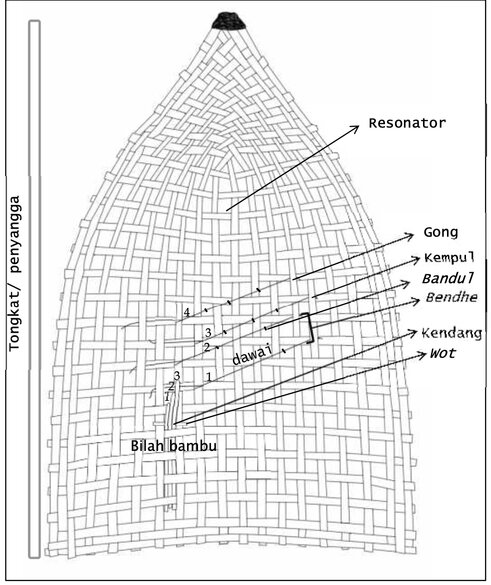
\includegraphics[width=8cm]{Gambar/strukturBundengan.jpg}
    \caption{Konstruksi alat musik \bundengan \cite{skripsiSaid}.}
    \label{fig:strukturBundengan}
\end{figure}
Dari penjelasan di atas, diketahui bahwa proses pembuatan \bundengan terdiri dari pembuatan \kowangan kemudian pemasangan komponen penghasil bunyi, yaitu senar dan bilah bambu. Bilah bambu yang biasa dipasang pada bagian kiri bawah \kowangan mewakili bunyi kendang, sedangkan senar raket badminton yang ditambahkan komponen \textit{bandulan} mewakili bunyi gamelan. Proses instalasi komponen senar dan bilah bambu ini menentukan keunikan bunyi yang dihasilkan \textit{bundengan} \cite{skripsiSaid}. Bilah bambu disisipkan berjajar pada kerangka \textit{kowangan} dengan penumpu dari bambu yang disebut \textit{wot}. Panjang dari bilah bambu yang dipetik menentukan seperti apa bunyi yang dihasilkan. Semakin panjang bilah yang dipetik maka bunyi yang dihasilkan akan memiliki frekuensi alami yang relatif rendah \cite{skripsiAzfar}. Senar dipasang membentang di dalam kerangka \textit{kowangan}, sedangkan ranting bambu atau \textit{bandulan} dipasang menggantung pada senar. Bunyi yang dihasilkan senar dipengaruhi oleh besarnya massa dan posisi \bandulan pada senar \cite{illusiveSound}. Biasanya jumlah \textit{bandulan} yang disematkan pada senar berjumlah satu buah untuk ketuk, dua buah untuk kenong, dua buah untuk kempul, dan tiga buah untuk gong. Seluruh konstruksi \bundengan dapat dilihat pada Gambar \ref{fig:strukturBundengan}.  \par 


%------new section


\section{Bunyi \textit{Bundengan}}
Ketika sebuah bunyi mencapai telinga pada sebuah pementasan musik, bunyi tersebut mengandung banyak sekali informasi. Manusia dapat merasakan tinggi rendahnya nada, tingkat kekerasan, dan warna bunyi \cite{meyer}. Ketika mendengar petikan senar \textit{bundengan}, sensasi yang dirasakan adalah seperti mendengar pementasan gamelan. Sensasi ini tidak lain disebabkan oleh konstruksi \bundengan itu sendiri. Selama beberapa tahun terakhir, berbagai penelitian telah dilakukan untuk mengetahui bagaimana bunyi yang unik ini bisa diproduksi oleh \textit{bundengan}. \par  

\subsection{Mekanisme Senar-\textit{Bandul}}
Pada tahun 2017, Parikesit dan Kusumaningtyas melakukan penelitian mengenai cara kerja komponen senar-\textit{bandul} menggunakan perekaman video berkecepatan tinggi dan pengamatan spektrum frekuensi melalui perekaman audio. Ketika senar dipetik, energi menjalar dari titik petikan senar menuju dua ujung senar \cite{bukuFletcher}. Ujung senar yang terikat akan memantulkan gelombang kembali. Namun karena massa \bandulan lebih besar dibanding massa senar, sebagian gelombang dipantulkan kembali oleh \textit{bandulan}. Dengan menggunakan perekaman berkecepatan tinggi diketahui bahwa massa \bandulan yang lebih besar meningkatkan inersia senar-\textit{bandul}. \textit{Bandulan} menghambat senar untuk mulai bergetar dan juga menghambat peluruhan getaran senar. \par 
Posisi \bandulan sepanjang senar menentukan bagaimana senar akan bergetar. \textit{Bandulan} membagi senar menjadi dua bagian, yaitu bagian yang lebih panjang dan yang lebih pendek. Senar bagian pendek memiliki durasi getar lebih lama, sedangkan senar bagian panjang bergetar pada frekuensi yang lebih tinggi. Perubahan posisi \bandulan mempengaruhi durasi getaran dari kedua bagian senar. Gambar \ref{fig:DataHighSpeed} memperlihatkan hasil pengukuran pengaruh perubahan posisi relatif \bandulan (posisi 0,5 menunjukkan titik tengah senar) terhadap perubahan durasi getaran dan frekuensinya. Ketika \bandulan digeser menuju bagian tengah senar, durasi getaran senar semakin lama dan frekuensi yang dihasilkan akan semakin kecil. Durasi getar yang lama dan berfrekuensi rendah ini yang menyerupai bunyi gong. \par 
\begin{figure}[t!]
    \centering
    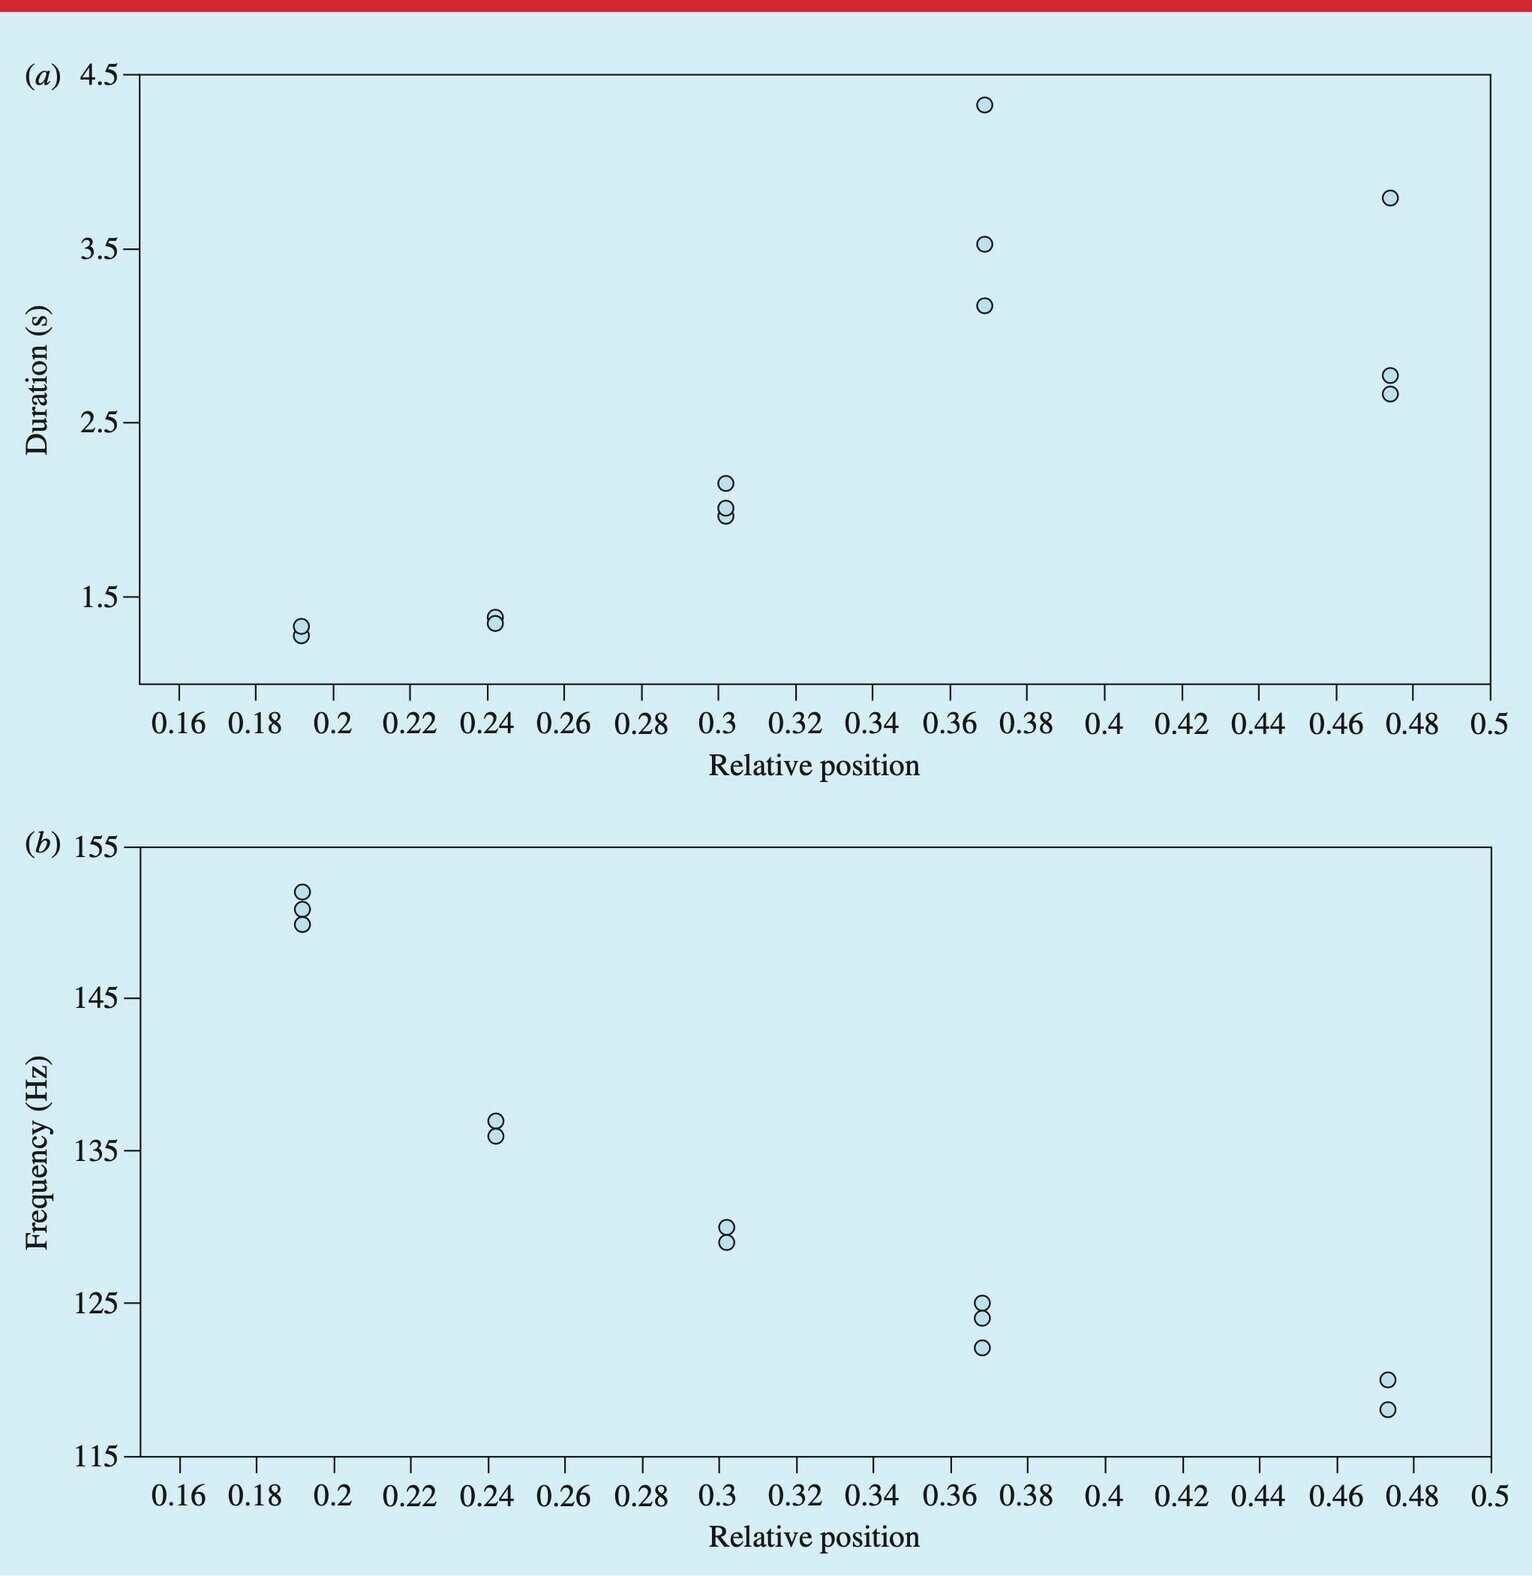
\includegraphics[width=13cm]{Gambar/highSpeedRecordData.jpg}
    \caption{Data hasil pengukuran: (a) Durasi getaran (dalam detik) sebagai fungsi posisi relatif \textit{bandulan}, (b) nilai frekuensi dengan amplitudo maksimum (dalam dB) sebagai fungsi posisi relatif \textit{bandulan} \cite{illusiveSound}.}
    \label{fig:DataHighSpeed}
\end{figure}   
Fenomena lain yang dirasakan ketika \bandulan digeser menuju bagian tengah senar adalah dirasakan adanya peningkatan nada oleh pendengaran, padahal kenyataannya tidak begitu \cite{illusiveSound}. Gambar \ref{fig:spektrumFrekPaperParikesit} memperlihatkan spektrum frekuensi dari lima sinyal audio untuk setiap posisi relatif \bandulan yang dijelaskan sebelumnya. Spektrum frekuensi tersebut menunjukkan setiap nilai frekuensi untuk berbagai puncak amplitudo dari setiap sinyal audio. Ketika \bandulan digeser menuju bagian tengah senar, senar bagian pendek akan menjadi lebih panjang dan begitu sebaliknya. Ketika senar bagian pendek menjadi lebih panjang dari sebelumnya, puncak frekuensi pertama ($\sim$75 Hz) dan kedua ($\sim$150 Hz) berubah menjadi lebih rendah. Ketika senar bagian panjang menjadi lebih pendek dari sebelumnya, puncak frekuensi ketiga ($\sim$225 Hz) dan keempat ($\sim$300 Hz) berubah menjadi lebih tinggi. Lantas mengapa jika ada peningkatan dan penurunan nilai frekuensi, telinga manusia hanya merasakan peningkatannya saja? Terdapat dua kemungkinan penjelasan terkait fenomena ini. 
\begin{figure}[t!]
    \centering
    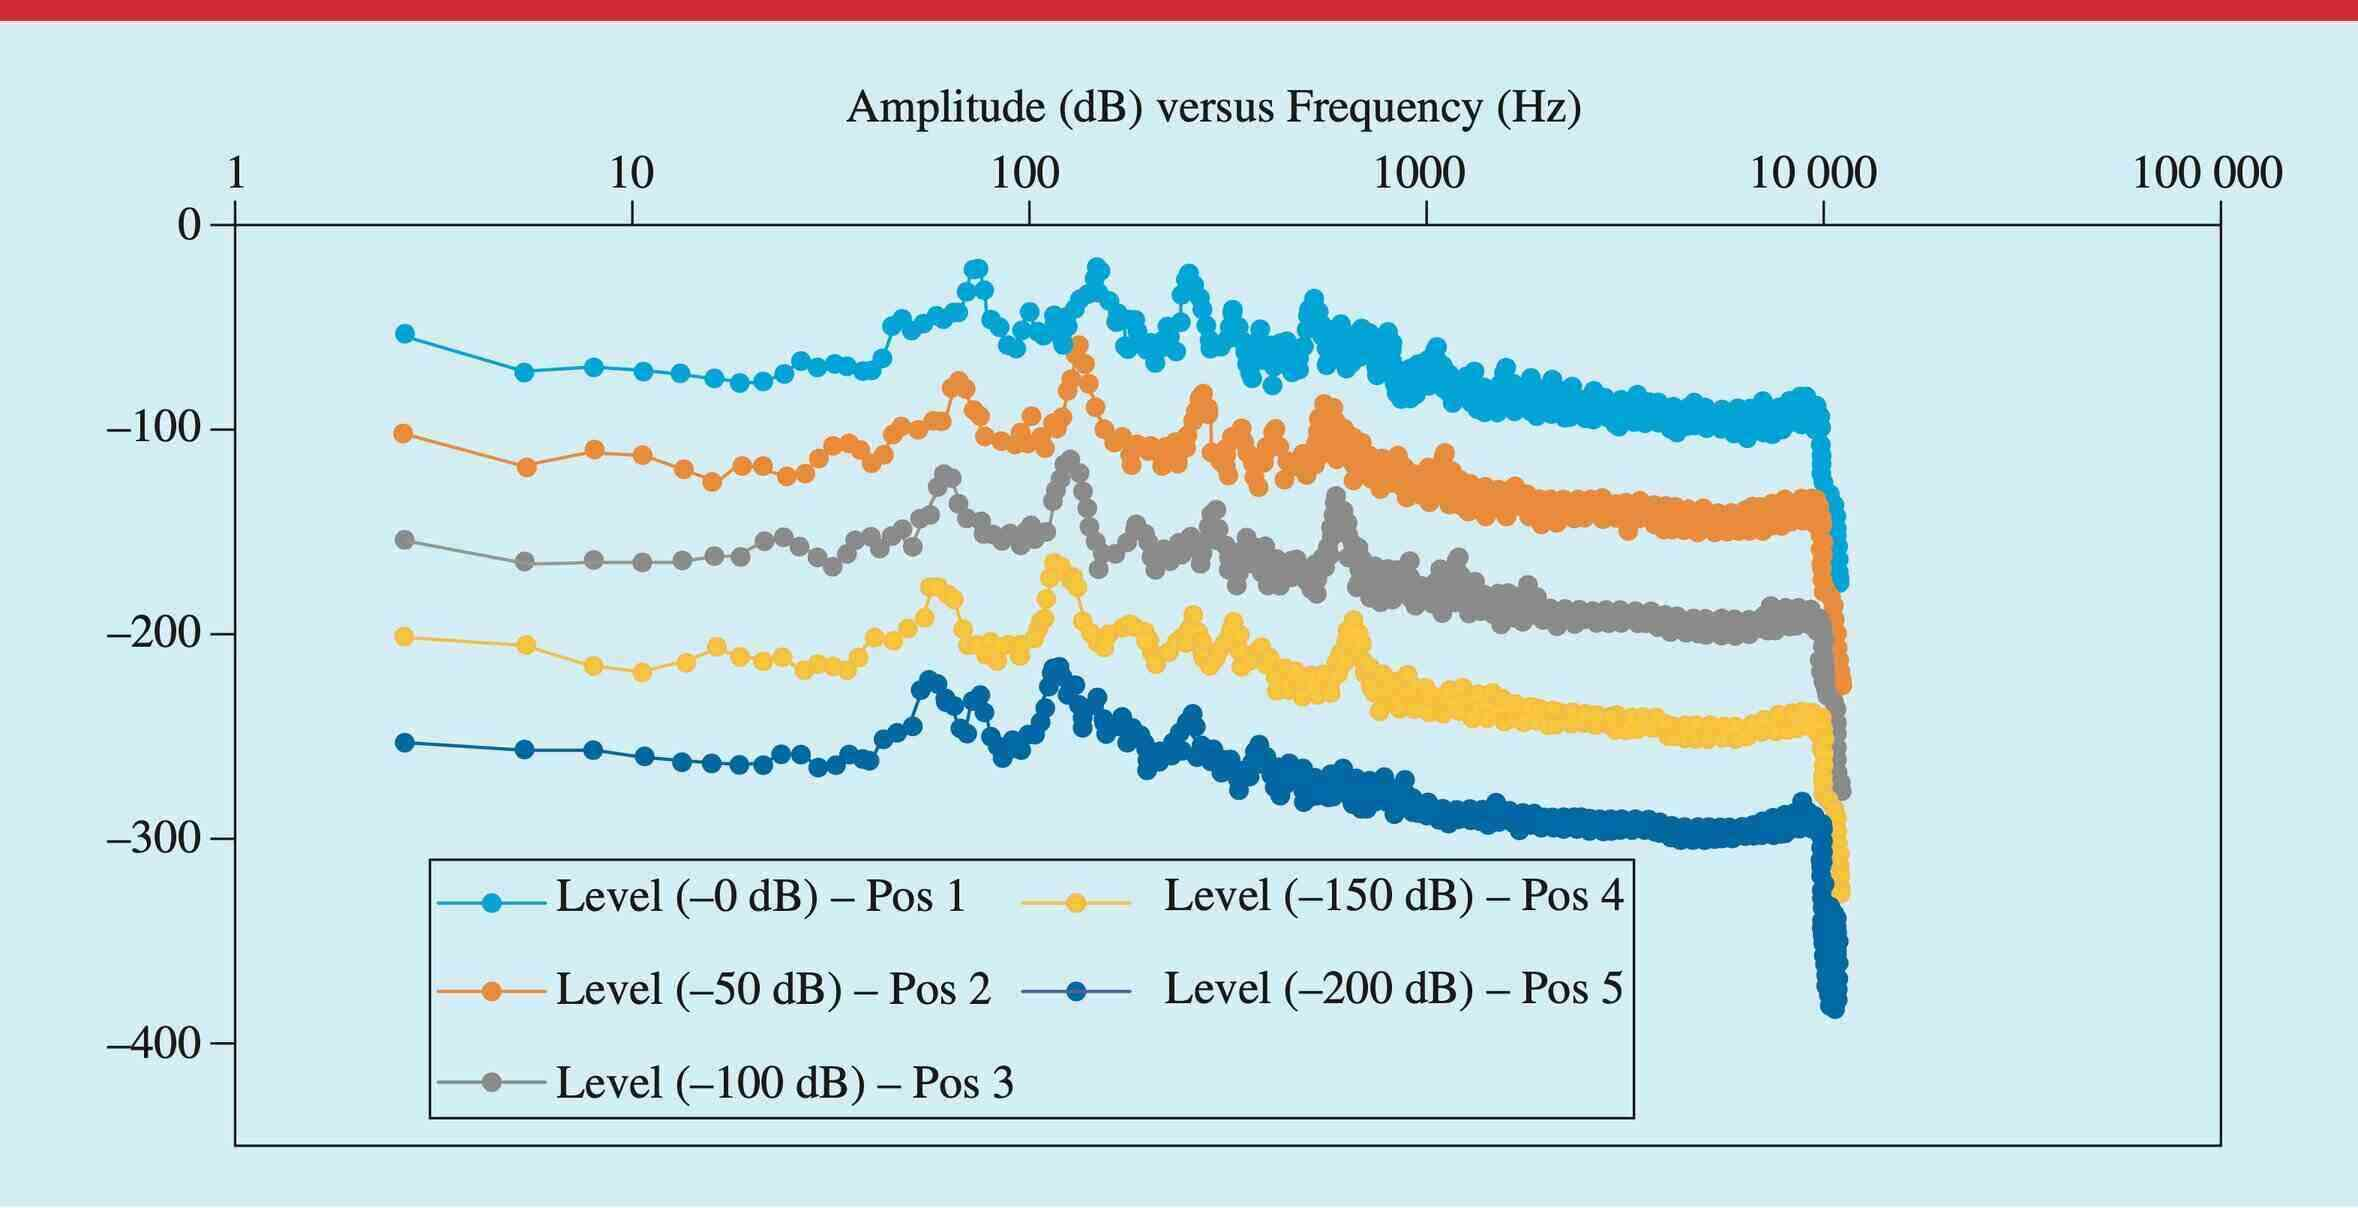
\includegraphics[width=14 cm]{Gambar/spektrumFrekPaperParikesit.jpg}
    \caption{Spektrum frekuensi untuk lima posisi relatif \bandulan pada senar \cite{illusiveSound}.}
    \label{fig:spektrumFrekPaperParikesit}
\end{figure}
\begin{enumerate}
    \item Terdapat waktu awal ketika alat musik memberi respon terhadap gaya masukan (dalam kasus ini adalah petikan senar). Waktu awal ini mengakibatkan getaran transien menjadi sinyal paling dominan yang dihasilkan alat musik. Getaran transien secara unik dapat menentukan warna bunyi atau \textit{timbre} dari setiap instrumen musik, seperti dapat dibedakannya bunyi gitar dan piano meskipun bunyi yang didengar berada pada nada yang sama. Jika meninjau lebih dekat pada hasil perekaman video berkecepatan tinggi, \bandulan tidak bergerak pada dua sampai tiga milisekon pertama setelah pemetikan. Pada saat itulah senar bagian panjang menghasilkan getaran dengan frekuensi tinggi, yang mana menentukan \textit{timbre} dari senar \textit{bundengan} \cite{illusiveSound}.
    \item Sistem pendengaran manusia tidak sepenuhnya sensitif terhadap seluruh frekuensi. Para insinyur menggunakan \textit{A-weighting curve} untuk menirukan respon alami dari pendengaran manusia, yang memiliki sensitivitas paling tinggi pada frekuensi kisaran 1 kHz-4 kHz. Oleh sebab itu, peningkatan puncak frekuensi ketiga dan keempat pada Gambar \ref{fig:spektrumFrekPaperParikesit} lebih mudah dirasakan daripada penurunan puncak frekuensi pertama dan kedua \cite{illusiveSound}.
\end{enumerate}

\textit{Bandulan} juga digunakan sebagai sarana pelarasan senar oleh para musisi \textit{bundengan}. Pelarasan ini dilakukan dengan menggeser-geser posisi \bandulan sampai tinggi nada yang diinginkan tercapai \cite{skripsiSaid}. Tidak menutup kemungkinan pula bahwa setiap senar \bundengan memiliki lebih dari satu buah \textit{bandulan}. Terkait hal ini, telah dilakukan penelitian mengenai pengaruh massa, posisi, dan jumlah \bandulan menggunakan simulasi komputer \cite{paperGetaranBandulan}. Hasil penelitian ini menunjukkan bahwa \bandulan adalah kunci dari terciptanya bunyi yang menyerupai alat musik metal gamelan. Jika massa \bandulan jauh lebih besar dibanding massa senar, getaran yang dihasilkan petikan senar akan berupa frekuensi non-harmonik. Hal ini serupa seperti instrumen perkusi logam yang juga memiliki spektrum non-harmonik. Jika terdapat dua \bandulan pada satu senar, spektrum frekuensi yang dihasilkan akan semakin rendah. Lebih daripada itu, ketika kedua \bandulan semakin digeser menuju bagian tengah senar maka nilai frekuensi fundamental semakin rendah dan cenderung mengarah ke nilai frekuensi tertentu \cite{paperGetaranBandulan}. \par 
\begin{figure}[t!]
    \centering
    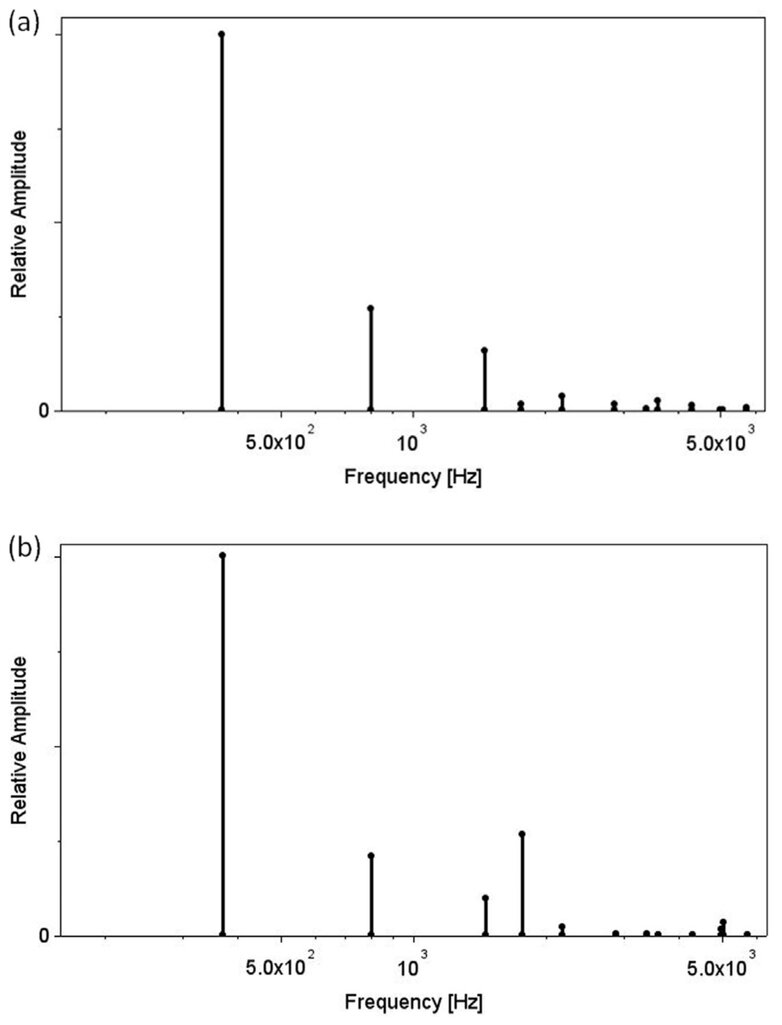
\includegraphics[width=8 cm]{Gambar/spekFrekBedaPetik.jpg}
    \caption{Spektrum frekuensi senar \bundengan dengan satu \bandulan pada posisi 0,06 m yang dipetik di (a) bagian panjang dan (b) bagian pendek \cite{paperGetaranBandulan}.}
    \label{fig:spekFrekBedaPetik}
\end{figure}
Pengamatan terhadap pengaruh massa, posisi, dan jumlah \bandulan tersebut dilakukan dengan mengamati senar \bundengan yang dipetik di tengah. Jika hanya terdapat satu buah \textit{bandulan} pada posisi 0,06 m, kemudian senar dipetik di titik tengah senar, petikan tersebut berada pada senar bagian panjang. Gambar \ref{fig:spekFrekBedaPetik}(a) memperlihatkan bagaimana amplitudo relatif dari setiap spektrum frekuensi ketika senar dipetik di tengah. Sedangkan ketika senar dipetik pada bagian pendek, spektrum frekuensi pada Gambar \ref{fig:spekFrekBedaPetik}(b) memperlihatkan amplitudo relatif yang berbeda. Tidak seperti ketika senar dipetik pada bagian panjang, mode getar ke-4 lebih kuat daripada mode getar ke-2 dan ke-3 pada senar yang dipetik di bagian pendek. Oleh sebab itu, pola getaran dengan frekuensi tinggi sekarang muncul pada bagian pendek senar. Dari sini didapat informasi bahwa getaran frekuensi tinggi selalu muncul pada bagian di mana senar tersebut dipetik, yang mana hal ini masuk akal karena di situlah energi eksitasi pertama kali diberikan \cite{paperGetaranBandulan}. \par
Meskipun demikian, simulasi mengenai pengaruh variasi massa, posisi, dan jumlah \bandulan beserta variasi titik petikan senar tersebut tidak mempertimbangkan dimensi dan orientasi dari \textit{bandulan}. Padahal, \textit{bandulan} yang menggantung pada senar \bundengan adalah benda tegar berbentuk tabung yang memiliki tinggi, diameter luar, dan diameter dalam \cite{skripsiMona}. Pengaruh dimensi dan orientasi \bandulan terhadap getaran ini kemudian diteliti dengan berbagai metode, baik melalui analisis mekanik \cite{skripsiMona}, simulasi komputer \cite{skripsiAyrton}, ataupun pengukuran secara langsung \cite{skripsiJulda}. Hasilnya, diketahui bahwa variasi nilai perbandingan tinggi-diameter ($h/d$) \bandulan pada senar tidak mempengaruhi nilai frekuensi fundamental getaran senar. Meskipun demikian, ketika nilai $h/d$ semakin besar atau dengan kata lain \bandulan semakin ramping, nilai frekuensi \overtone getaran senar akan semakin mengecil \cite{prosidingDimensiBandulan}. Frekuensi \overtone adalah frekuensi alami yang nilainya lebih besar dari frekuensi fundamental. \par 

\subsection{\textit{Kowangan} sebagai Resonator \textit{Bundengan}}\label{sub-subBab:kowanganResonator}
Selain senar-\bandul dan bilah bambu, \bundengan juga tersusun dari \textit{soundboard} berbentuk perisai, yaitu \textit{kowangan}. Terkait hal ini, telah dilakukan pembuatan simulator oleh Christianto pada tahun 2018 \cite{skripsiRaymond}. Simulator ini telah dapat menunjukkan bagaimana distribusi TTB pada bagian depan \textit{kowangan} dengan menghitung bagaimana dinding-dinding \kowangan memancarkan bunyi ke depan. Meskipun demikian, simulator yang dibangun ini masih sangat sederhana, bentuk konstruksinya (Gambar \ref{fig:modelKowanganRaymond}) belum merepresentasikan wujud \kowangan yang sesungguhnya. \par 
\begin{figure}[t!]
    \centering
    \subfigure[]{\label{fig:tampakKiriRaymond}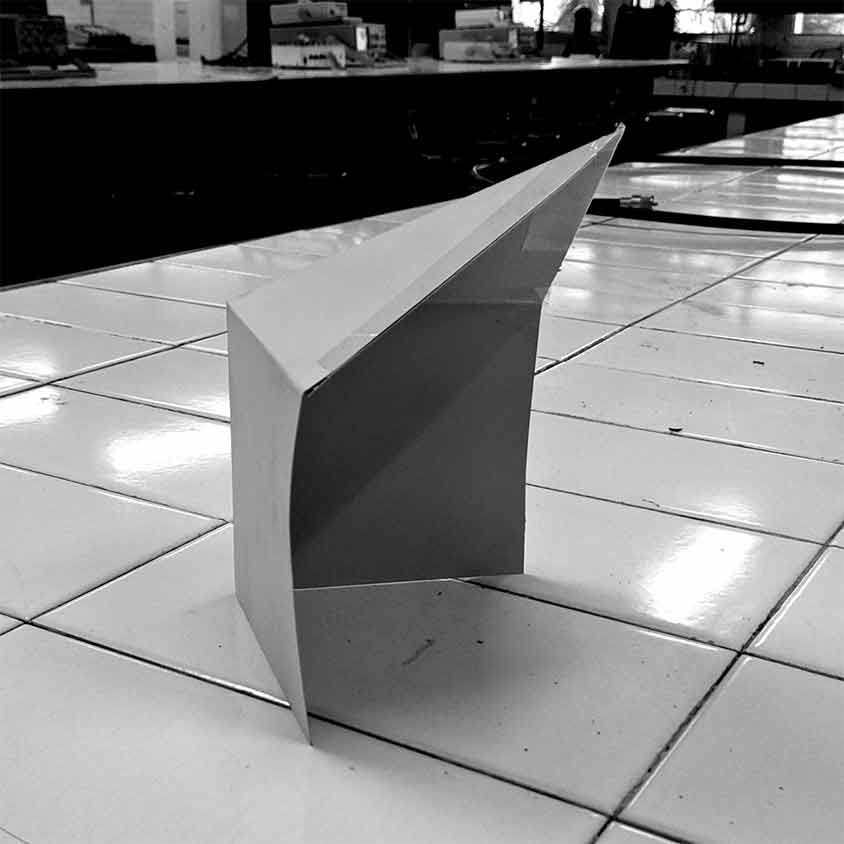
\includegraphics[width=50mm]{Gambar/tampakKananRaymond.jpg}}
    \hspace{1 cm}
    \subfigure[]{\label{fig:tampakKananRaymond}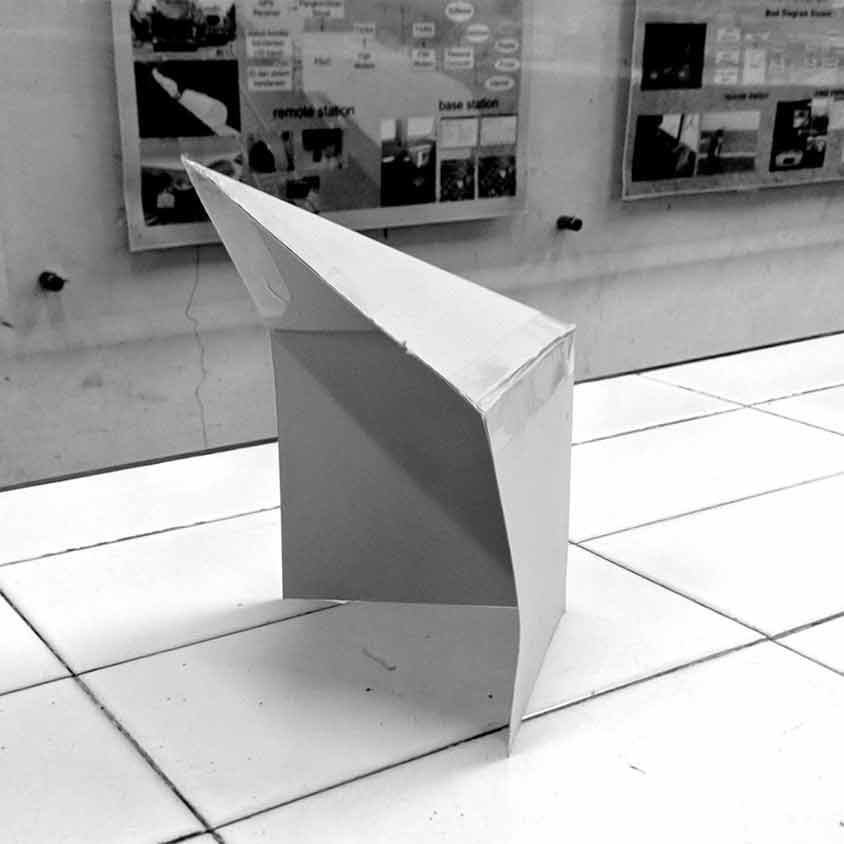
\includegraphics[width=50mm]{Gambar/tampakKiriRaymond.jpg}}
    \caption{Model fisik \textit{kowangan}; (a) tampak kiri dan (b) tampak kanan \cite{skripsiRaymond}.}
    \label{fig:modelKowanganRaymond}
\end{figure}
Pada tahun 2019, Simanungkalit melakukan penelitian terkait getaran pada \kowangan menggunakan metode eksperimental \cite{skripsiSimanungkalit}. Penelitian dilakukan menggunakan \textit{impact hammer} sebagai pemberi gaya impuls dan \textit{accelerometer} yang keduanya terhubung pada osiloskop digital untuk dianalisis. Pada awalnya penelitian dilakukan untuk 10 titik pengukuran dengan 10 kali pengulangan, namun hasil analisis menunjukkan amplitudo frekuensi pada titik ke-5 berbeda cukup jauh jika dibandingkan dengan titik ukur lain. Selain itu, terdapat perbedaan nilai frekuensi yang signifikan untuk titik-titik ukur yang berdekatan. Oleh sebab itu, dilakukan pengamatan untuk 19 titik ukur dengan 20 kali pengulangan, dengan harapan nilai rata-rata frekuensi yang terukur dapat lebih seragam. Tabel \ref{tab:getaranKowangan} memperlihatkan data frekuensi alami dari \kowangan beserta nilai deviasi standarnya. Karena nilai deviasi standar yang tinggi, nilai rata-rata frekuensi ini tidak dapat merepresentasikan frekuensi alami \textit{kowangan} sebenarnya. \par 
\begin{table}[h!]
    \centering
    \caption{Hasil pengukuran frekuensi getaran \kowangan pada 19 titik ukur dengan 20 kali pengulangan \cite{skripsiSimanungkalit}.}
    \begin{tabular}{m{3 cm} l l}
        \hline
        Frekuensi & \multirow{2}{3cm}{Frekuensi rata-rata (Hz)} & \multirow{2}{3cm}{Deviasi Standar (Hz)} \\
        alami ke- & & \\
        \hline
        1 & 1068,1 & 225,1 \\
        2 & 1150,3 & 192,9 \\
        3 & 1202,5 & 195,8 \\
        \hline
    \end{tabular}
    \label{tab:getaranKowangan}
\end{table}
Kemudian pada tahun 2020, Parikesit melakukan studi mengenai pemfokusan bunyi musik \bundengan pada \textit{kowangan} \cite{alatMusikPersonal}. Penelitian ini dilakukan dengan terlebih dahulu mempelajari bagaimana proses \kowangan dibuat untuk selanjutnya dibuat model \kowangan menggunakan simulasi komputer. Tidak seperti pada simulator yang dibangun Christianto, bentuk kelengkungan \kowangan pada model yang dibuat ini sudah cukup menyerupai aslinya. Dalam menganalisis radiasi bunyi pada model \textit{kowangan}, elemen akustik dari \kowangan dimodelkan sebagai sumber dipol. Hasilnya menunjukkan bahwa sumber dipol ini mengarah pada titik yang sama, yaitu bagian tengah struktur model \textit{kowangan}. Gambar \ref{fig:fokusSuaraKowangan} memperlihatkan beberapa sumber dipol pada model \textit{kowangan}. Hasil ini tentu membuktikan kebenaran bahwasanya alat musik \bundengan lebih baik jika dinikmati secara pribadi.
\begin{figure}[t!]
    \centering
    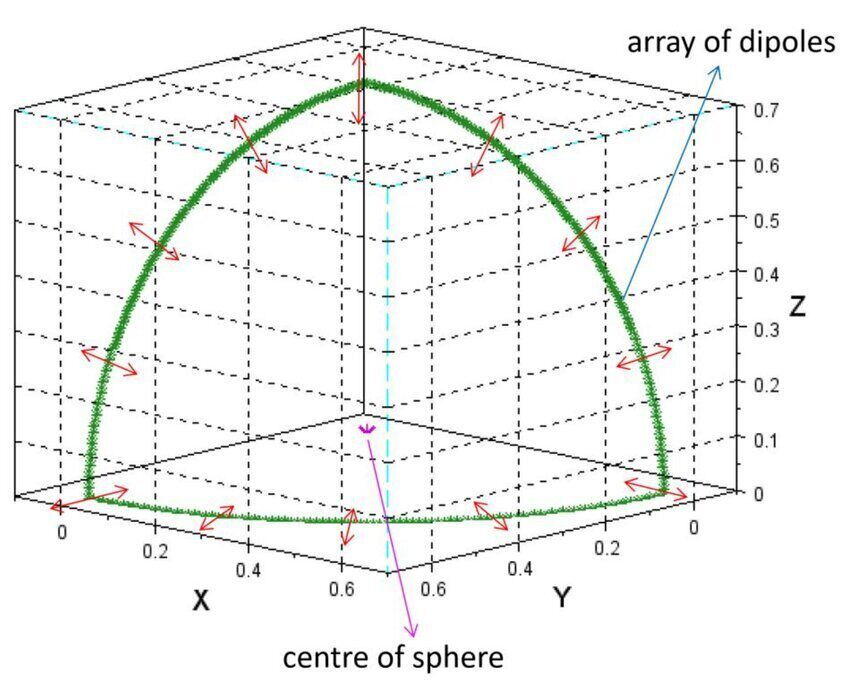
\includegraphics[width=8 cm]{Gambar/fokusSuaraKowangan.jpg}
    \caption{Pemfokusan bunyi pada bentuk dasar perisai \kowangan \cite{alatMusikPersonal}.}
    \label{fig:fokusSuaraKowangan}
\end{figure}


%--------------new section-----------%

\section{Direktivitas \textit{Bundengan}}
Karena simulator yang dibangun oleh Christianto masih jauh dari bentuk asli \textit{kowangan} (Gambar \ref{fig:modelKowanganRaymond}), simulasi distribusi nilai TTB pada \kowangan tersebut belum bisa dikatakan sesuai. Untuk mengetahui sebaran nilai TTB dengan lebih realistis, perlu dilakukan pengukuran secara langsung. Pada tahun 2019, Muharram melakukan pengukuran TTB di depan \bundengan pada bidang datar dengan variasi jarak 1 m dan 2 m \cite{skripsiMuharram}. \Bundengan yang diukur terdiri dari lima senar. Setiap senar diukur nilai TTB-nya untuk kedua variasi jarak tersebut. Hasil pengukuran untuk jarak pengukuran 1 m menunjukkan nilai TTB yang tinggi pada bagian tengah untuk seluruh senar. Untuk pengukuran pada jarak 2 m, nilai TTB senar 1 dan 2 memiliki nilai yang cenderung tinggi, sedangkan senar 3, 4, dan 5 nilai TTB-nya cenderung rendah. \par 
Meskipun pengukuran nilai TTB \bundengan telah berhasil dilakukan, namun hasil pengukuran tersebut sangat terbatas untuk diubah parameter-parameternya. Sebagai contoh, terdapat kesulitan jika ingin mengukur nilai TTB dengan variasi dimensi \kowangan ataupun susunan senar yang berbeda. Untuk mendapatkan nilai distribusi bunyi yang universal dengan berbagai variasi parameter, cukup sulit jika menggunakan metode eksperimental, karena metode ini akan sangat memakan waktu dan biaya dalam pengerjaannya. Oleh sebab itu, metode simulasi komputer adalah metode alternatif yang dapat dipilih. Bentuk \kowangan pada simulator yang dibangun oleh Christianto \cite{skripsiRaymond} telah diperbarui oleh Parikesit sehingga bentuknya lebih menyerupai \kowangan sesungguhnya. Gambar \ref{fig:fokusSuaraKowanganSamping} memperlihatkan bentuk model \kowangan dengan bentuk dasar seperdelapan bola. Seperti yang telah dijelaskan pada sub-subbab \ref{sub-subBab:kowanganResonator}, selain memperbarui bentuk \kowangan Parikesit juga menghitung bagaimana elemen pada model \kowangan tersebut bergetar secara transversal dengan dimodelkan sebagai sumber dipol. \par 
\begin{figure}[t!]
    \centering
    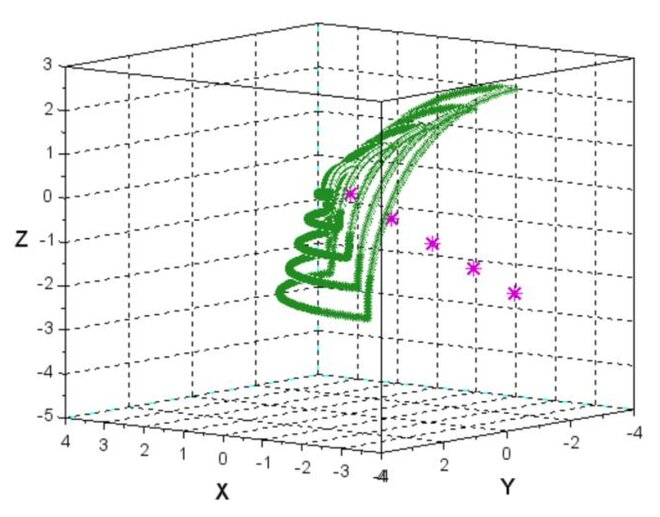
\includegraphics[width= 8 cm]{Gambar/fokusSuaraKowanganSamping.jpg}
    \caption{Bentuk \kowangan yang telah diperbarui dengan bentuk dasar seperdelapan bola \cite{alatMusikPersonal}.}
    \label{fig:fokusSuaraKowanganSamping}
\end{figure}
Simulasi yang dilakukan Parikesit menggunakan model \kowangan terbaru tersebut belum menyimulasikan bagaimana bunyi musik \bundengan merambat. Oleh sebab itu, Wijanarko pada tahun 2020 membuat kembali simulator dengan bentuk dasar yang telah diperbarui, yaitu bentuk seperdelapan bola \cite{skripsiZidan}. Penelitian ini kemudian membandingkan hasil perambatan bunyi dengan hasil yang didapat simulator Christianto dan dengan hasil pengukuran Muharram. Dalam proses pembangunan simulator tersebut, diketahui bahwa model terbaru buatan Parikesit memiliki kerapatan sumber bunyi yang tidak seragam. Karena hal ini, perlu dilakukan modifikasi terhadap model \kowangan Parikesit. Simulator yang berhasil dibangun ini menghasilkan pola distribusi TTB yang serupa dengan simulator milik Christianto, tetapi pada jarak pengukuran yang berbeda. Jika dibandingkan dengan hasil pengukuran eksperimental Muharram, simulator ini dapat merepresentasikan bunyi frekuensi rendah dan jarak pengukuran yang relatif jauh. Meskipun demikian, simulator ini belum dapat merepresentasikan bunyi frekuensi tinggi dan jarak pengukuran yang relatif dekat. \par 
Pengukuran TTB yang telah dilakukan baik melalui pengukuran langsung maupun menggunakan simulator hanya berhasil mendapatkan nilai TTB untuk area di depan \textit{kowangan}. Padahal, jika dikaitkan dengan masalah pada pementasan musik \textit{bundengan}, diperlukan nilai TTB untuk berbagai arah rambat bunyinya. Dengan kata lain perlu dilakukan pengukuran terhadap direktivitas \textit{bundengan}. Pada tahun 2020, Kusumaningtyas, Christianto, dan Parikesit melakukan pengukuran direktivitas dari dua \bundengan yang berbeda \cite{prosidingDirektivitas}, yaitu:
\begin{enumerate}
    \item \Bundengan pertama dibuat dan dimainkan oleh musisi senior. \Bundengan ini memiliki empat buah senar.
    \item \Bundengan yang kedua dibuat dan dimainkan oleh musisi yang lebih muda. \Bundengan ini memiliki delapan senar.
\end{enumerate}
Kedua \bundengan terbuat dari material yang sama. Sedangkan pelarasan senar kedua \bundengan dilakukan oleh masing-masing musisi, namun sama-sama mengacu ke bunyi gamelan Wonosobo. Perekaman bunyi dan pengukuran dilakukan pada ruangan \textit{semi-anechoic}. Perekaman bunyi dilakukan untuk setiap arah 30º menggunakan tujuh mikrofon kondensor, seperti yang ditunjukkan pada Gambar \ref{fig:bundenganBatasanMasalah}. Untuk mendapatkan pengukuran pada semua arah (360º), dilakukan dua kali pengukuran dengan memutar posisi \textit{bundengan}. \par  
Hasil pengukuran disajikan dalam spektrum warna sebagai penunjuk nilai TTB untuk setiap variasi arah (yang ditunjukkan sumbu tegak) dan untuk variasi frekuensi (yang ditunjukkan sumbu datar). Tidak seperti hasil pengukuran nilai TTB pada penelitian-penelitian sebelumnya, hasil pengukuran ini tidak hanya menampilkan frekuensi fundamental saja, namun juga dapat memperlihatkan frekuensi \textit{overtone} dari setiap senar \textit{bundengan}. Meskipun demikian, frekuensi \textit{overtone} hanya terlihat jelas pada senar \Bundengan 2. Sedangkan senar 1 dan 2 pada \bundengan 1 terlihat hanya memiliki satu frekuensi fundamental yang nilai TTB-nya paling kuat. Untuk senar 3 dan 4 pada \bundengan 1 terlihat frekuensi \overtone yang samar namun sudah cukup kuat untuk diamati. Selain itu, karena kedua \bundengan memiliki jumlah senar yang berbeda, rentang nada yang dapat dihasilkan juga berbeda. Tidak semua senar pada \bundengan 2 memiliki padanan frekuensi fundamental yang sama dengan senar pada \bundengan 1. Sebagai contoh, tidak ada senar pada \bundengan 1 yang frekuensi fundamentalnya cukup tinggi untuk dibandingkan dengan senar 1, 2, dan 3 pada \bundengan 2. Meski begitu, terdapat tiga senar \bundengan 1 yang frekuensi fundamentalnya bernilai hampir sama dengan tiga senar \bundengan 2. Tabel \ref{tab:prosidingDirektivitas} memperlihatkan perbandingan direktivitas ketiga senar dari masing-masing \bundengan dengan nilai frekuensi fundamental yang cukup dekat. \par 
\begin{table}[t!]
    \centering
    \caption{Perbandingan nilai direktivitas senar 1, 2, dan 3 pada \bundengan 1 dengan senar 4, 6, 8 pada \bundengan 2 yang memiliki nilai frekuensi fundamental cukup dekat \cite{prosidingDirektivitas}.}
    \begin{tabular}{c c}
        \hline
        \textbf{\Bundengan 1} & \textbf{\Bundengan 2} \\
        \hline
        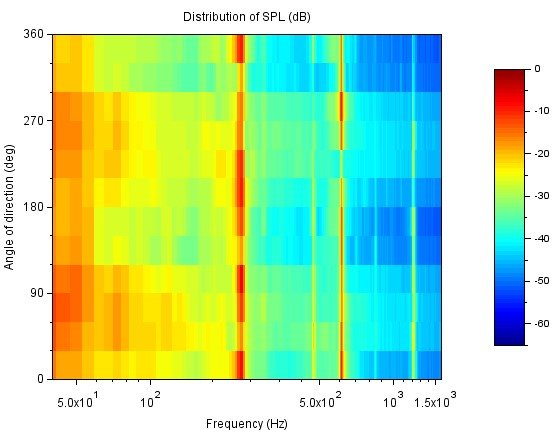
\includegraphics[width=65mm]{Gambar/senar1yangA.jpg} & 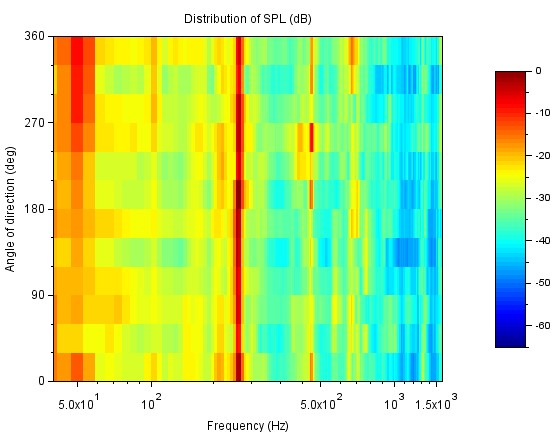
\includegraphics[width= 65mm]{Gambar/senar4yangB.jpg}\\
        Senar 1, $f_1=233$ Hz & Senar 4, $f_1=225$ Hz \\
        \hline
        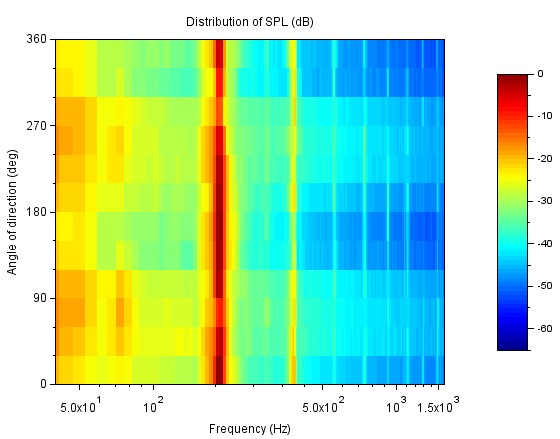
\includegraphics[width=65mm]{Gambar/senar2yangA.jpg} & 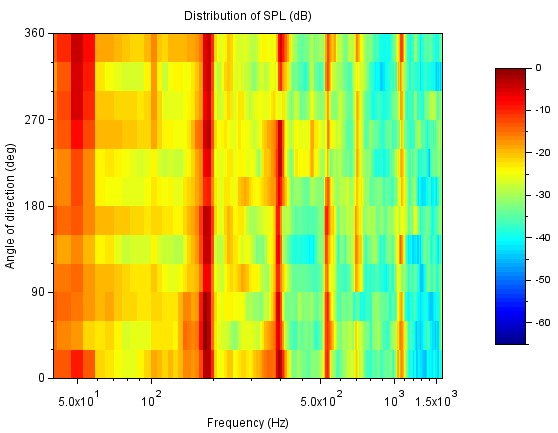
\includegraphics[width=65mm]{Gambar/senar6yangB.jpg}\\
        Senar 2, $f_1=184$ Hz & Senar 6, $f_1=166$ Hz \\
        \hline
        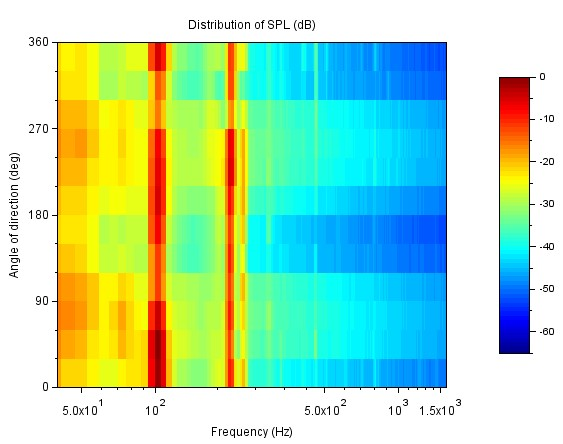
\includegraphics[width=65mm]{Gambar/senar3yangA.jpg} & 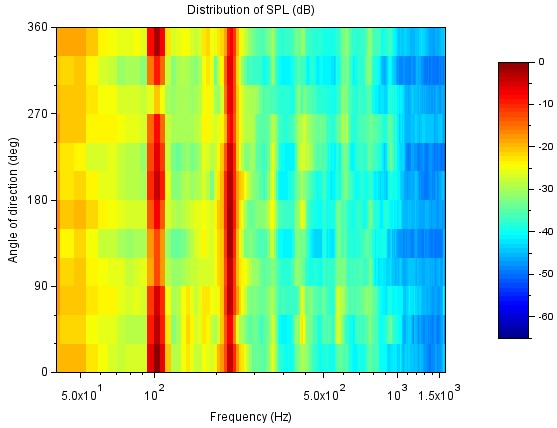
\includegraphics[width=65mm]{Gambar/senar8yangB.jpg}\\
        Senar 3, $f_1=99$ Hz & Senar 8, $f_1=100$ Hz \\
        \hline
    \end{tabular}
    \label{tab:prosidingDirektivitas}
\end{table}
\newpage
\paragraph{}
\newpage
Kedua \bundengan secara konsisten menghasilkan frekuensi fundamental dengan pola direktivitas yang menunjukkan nilai TTB paling tinggi pada arah 0 dan 180 derajat \cite{prosidingDirektivitas}. Meskipun demikian, kedua \bundengan menghasilkan pola direktivitas yang berbeda untuk frekuensi \textit{overtone}-nya. Fenomena ini menunjukkan bahwa kemiripan pola direktivitas pada frekuensi fundamental disebabkan oleh bentuk dasar dan ukuran yang sama. Sedangkan perbedaan pola direktivitas pada frekuensi \overtone terjadi karena kemungkinan perbedaan pada ketepatan dimensi \textit{bundengan}, kelengkungan \textit{kowangan}, dan ketepatan peletakan senar pada anyaman bambu \textit{kowangan}. Dari hasil yang telah dipaparkan, dapat disimpulkan bahwa setiap pendengar musik \bundengan pada sebuah pementasan akan merasakan pengalaman yang berbeda-beda tergantung dari lokasi tempat duduk. \par 

%-----new section

\section{Visualisasi Data Akustika Musik}
Notasi musik yang dikenal saat ini merupakan sistem visualisasi yang telah dikembangkan sejak lebih dari 10 abad yang lalu. Dahulu pada tahun 900 Masehi, anggota paduan suara di biara Italia mempelajari nyanyian gereja dengan menirukan setiap interval melodi yang diajarkan hanya dengan mengandalkan telinga \cite{GuidoArezzo}. Selain itu, para anggota juga perlu menyamakan dengan tepat tinggi nada atau \textit{pitch} yang dimainkan oleh instruktur paduan suara. Tentu metode pembelajaran ini akan sulit diingat. Jika anggota paduan suara mulai mempelajari nyanyian baru, mereka perlu mempelajari ulang nyanyian lama jika hendak menampilkannya beberapa tahun kemudian. \par 
Sekitar tahun 1025, seorang biarawan bernama Guido pindah ke kota bernama Arezzo. Dalam kunjungannya ke berbagai biara, Guido mengamati betapa sulitnya para penyanyi muda berusaha mempelajari nyanyian gereja. Guido pun terpikir untuk membuat sebuah alat yang dapat memudahkan seseorang dalam bernyanyi. Pada masa itu, para penyanyi dibantu dengan menggunakan \textit{neumes}, yaitu sebuah simbol notasi yang merepresentasikan kontur musik. Pada Gambar \ref{fig:neumes} diperlihatkan salah satu contoh notasi \textit{neumes}. Meskipun demikian, \textit{neumes} hanya menyatakan jumlah nada dan arah melodi keseluruhan tanpa menjelaskan \textit{pitch} secara spesifik dan interval antar nada. \par 
\begin{figure}[t!]
    \centering
    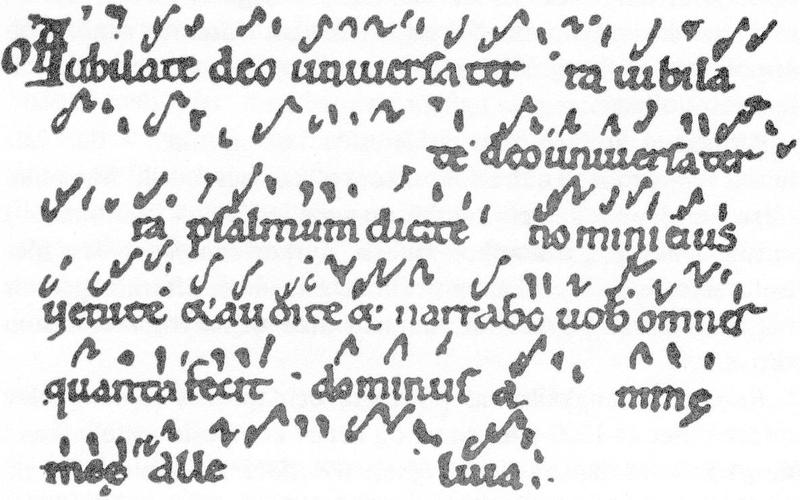
\includegraphics[width=10cm]{Gambar/Neume2.jpg}
    \caption{Salah satu penggalan nyanyian gereja dengan notasi \textit{neumes} di setiap bagian atas kata \cite{WQXR}.}
    \label{fig:neumes}
\end{figure}
Oleh sebab itu, Guido kemudian terpikir sebuah sistem penulisan yang lebih dapat membantu para penyanyi, yaitu dengan menambahkan \textit{the staff} atau dalam bahasa Indonesia disebut paranada pada notasi \textit{neumes} \cite{WQXR}. Paranada seperti yang diperlihatkan pada Gambar \ref{fig:neum4garis} terdiri dari empat garis yang salah satunya terdapat sebuah "kunci" yang mengindikasikan posisi \textit{pitch} referensi. Dengan begitu, para anggota paduan suara dapat lebih mudah mendeteksi tingkat \textit{pitch} yang dimainkan, atau dengan kata lain membaca musik \cite{WQXR}. \par
Notasi \textit{neumes} yang dimodifikasi oleh Guido memang sudah lebih baik, namun belum dapat menjelaskan seberapa lama nada tersebut harus dimainkan. Masalah ini kemudian dipecahkan oleh notasi \textit{mensural} \cite{WQXR}. Notasi \textit{mensural} biasa digunakan untuk vokal musik sekuler, di mana notasi ini menggunakan lima buah garis paranada. Pada Gambar \ref{fig:notasimensural} diperlihatkan salah satu contoh penulisan notasi \textit{mensural}. Dapat diamati dengan sangat jelas penggunaan lima garis paranada dan simbol-simbol yang digunakan sangat mirip dengan notasi musik modern saat ini. \par 
\begin{figure}[t!]
    \centering
    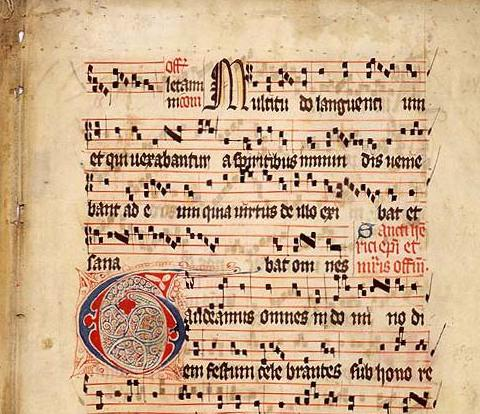
\includegraphics[width=9cm]{Gambar/Graduale_Aboense.jpg}
    \caption{\textit{Neumes} dengan empat garis paranada \cite{WQXR}.}
    \label{fig:neum4garis}
\end{figure}
\begin{figure}[b!]
    \centering
    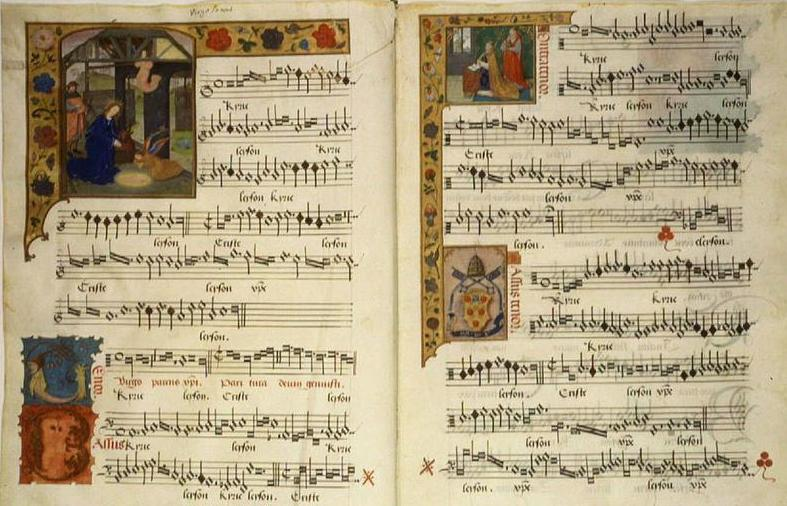
\includegraphics[width=13.5cm]{Gambar/1015px-Barbireau_illum.jpg}
    \caption{Contoh penulisan notasi \textit{mensural} \cite{WQXR}.}
    \label{fig:notasimensural}
\end{figure}
Yang-Hann Kim, seorang Professor dari Korea Advanced Institute of Science and Technology mengungkapkan pentingnya penggambaran visual mengenai \textit{sound field} atau direktivitas ketika proses pembelajaran akustika. Untuk menyajikan hal ini, biasanya diperlukan peralatan yang cukup rumit seperti susunan mikrofon dan alat pemindai. Hawley dan McClain pada tahun 2018 mengembangkan sebuah piranti lunak berbasis sistem operasi iOS yang dapat dijadikan metode sederhana dalam menyajikan data direktivitas \cite{PakeHP}. Prinsip kerja dari piranti lunak ini adalah dengan mengandalkan sensor yang tersedia pada ponsel pintar, kemudian piranti ini secara otomatis akan menampilkan pola direktivitas pada diagram polar.  \par 
Selain menggunakan mikrofon internal, pengukuran juga dapat menggunakan mikrofon eksternal yang dipasang melalui \textit{audio jack}. Radius dari diagram polar yang dihasilkan mewakili TTB sedangkan sudutnya mewakili orientasi ponsel sekaligus sensor. Grafik diagram polar ini memungkinkan untuk ditampilkan langsung ataupun diunduh dalam format CSV. Pada percobaan pengukuran, digunakan ponsel iPhone 5s yang diletakkan di atas pengeras suara berjenis Mackie HR824mk2. Pada Gambar \ref{fig:contohPolarplotter} diperlihatkan pola direktivitas yang ditampilkan dalam diagram polar untuk beberapa variasi frekuensi dan lokasi pengukuran. \par
\begin{figure}[h!]
    \centering
    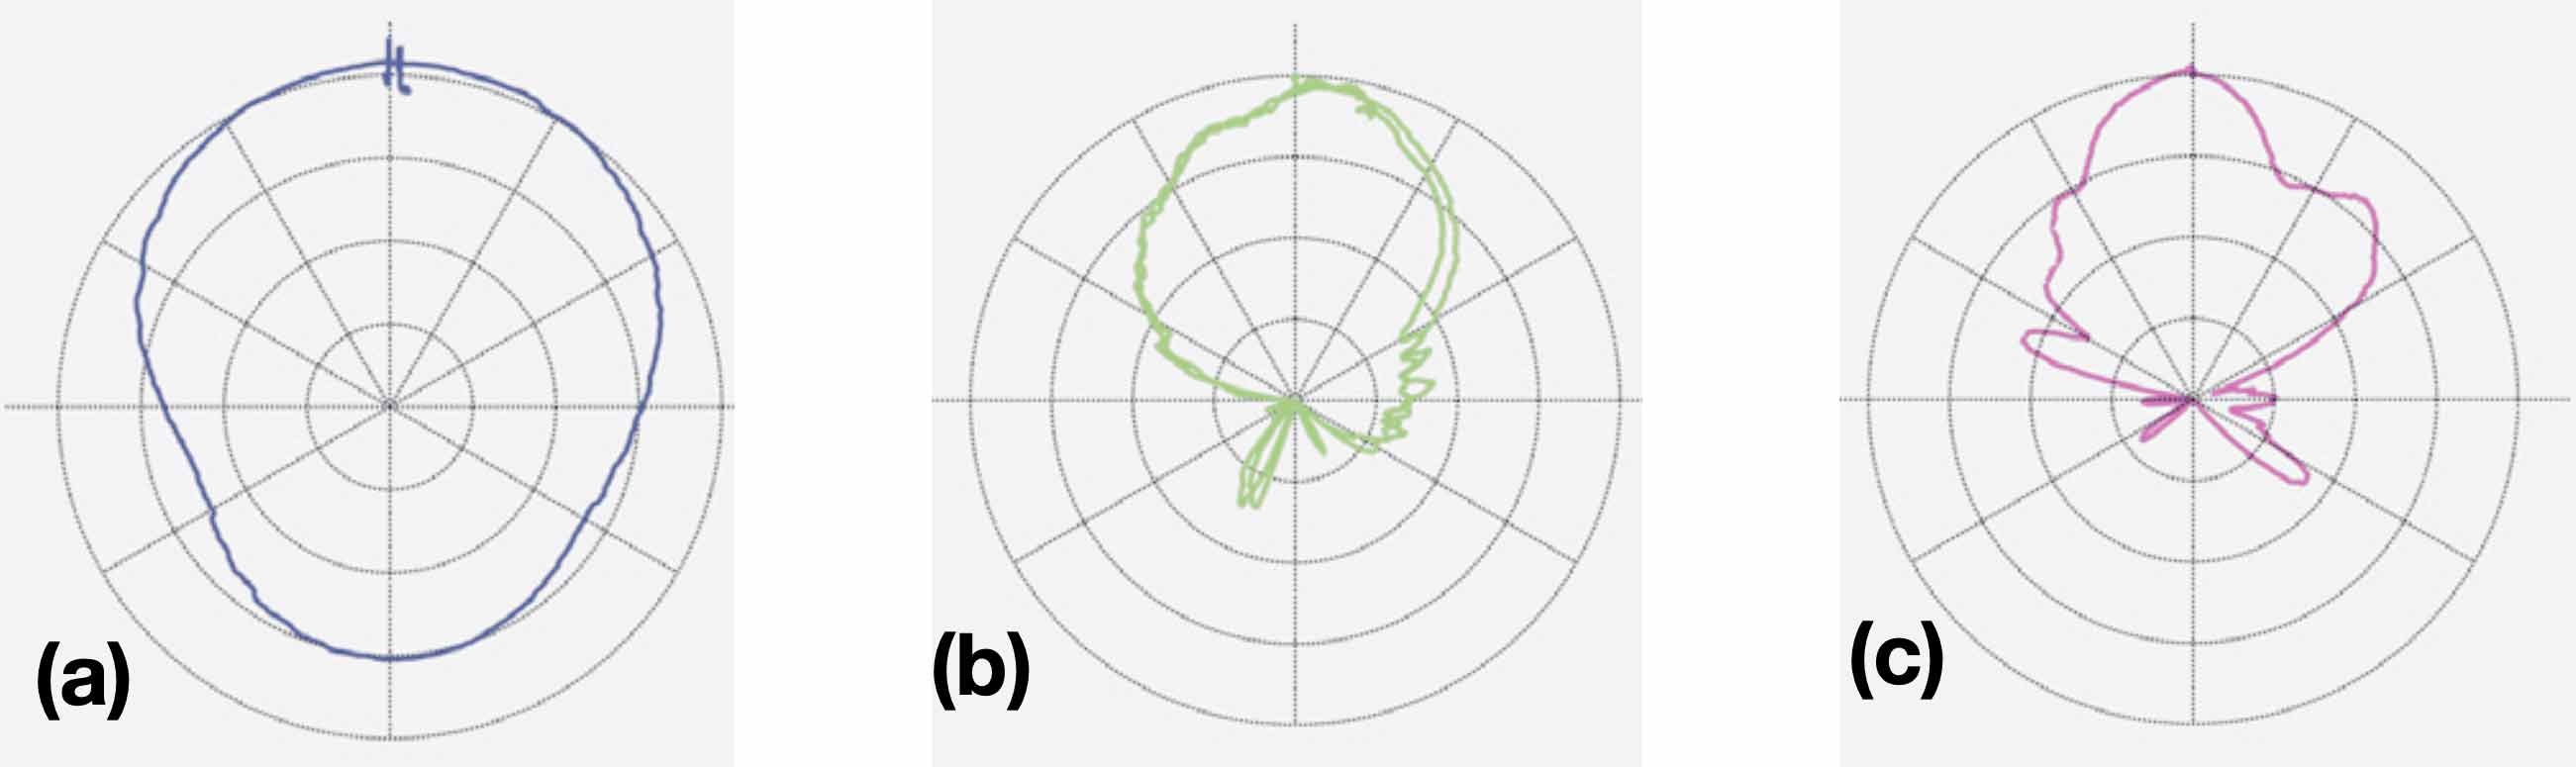
\includegraphics[width=14cm]{Gambar/ContohPolarPlotter.jpg}
    \caption{Diagram polar untuk pengukuran direktivitas bunyi pada frekuensi (a) 250 Hz dan (b) 4 kHz diukur di luar ruangan, lalu (c) 4 kHz untuk perekaman pada ruang kelas yang dapat terjadi pemantulan bunyi \cite{PakeHP}.}
    \label{fig:contohPolarplotter}
\end{figure}
\newpage
Meskipun hanya terbatas pada sistem operasi iOS, piranti lunak ini telah mampu mengatasi keterbatasan waktu serta perangkat perekaman. Pengamatan mengenai pola direktivitas menjadi lebih mudah untuk diperkenalkan kepada para siswa. Grafik yang disajikan dari hasil pengukuran ini dapat menggambarkan seperti apa bunyi yang akan dirasakan telinga pada setiap posisi tertentu. Dengan begitu para siswa dapat dengan mudah bereksplorasi terkait berbagai sumber bunyi dan bagaimana bunyi tersebut merambat ke segala arah.  \par 
Dua inovasi yang telah dipaparkan di atas adalah contoh dari perkembangan visualisasi data di bidang musik dan akustika. Baik pada abad pertengahan maupun era modern, visualisasi yang tepat serta metode yang mudah sangat dibutuhkan dalam pembelajaran. Ketika proses pembelajaran menjadi lebih mudah diakses, peluang menuju inovasi ataupun pemecahan masalah yang lebih besar akan semakin dekat. Hal ini selaras dengan tujuan dari sistem visualisasi data direktivitas \bundengan yang hendak dibangun penulis juga bertujuan untuk membantu para musisi serta pegiat \bundengan dalam proses pengolahan informasi menuju pemecahan masalah yang jauh lebih besar. \par 

%----new section

\section{Kontribusi Penelitian Penulis}
Penelitian mengenai distribusi bunyi \bundengan mengarah pada penyelesaian masalah mengenai pementasan musik \textit{bundengan}. Data direktivitas \bundengan yang telah diukur oleh Kusumaningtyas, Christianto, dan Parikesit telah dapat merepresentasikan dengan baik perambatan bunyi \bundengan ke segala arah \cite{prosidingDirektivitas}. Setiap rencana penyelesaian masalah kesenian yang disusun oleh para insinyur selalu memerlukan kerja sama dan komunikasi dengan pegiat seni itu sendiri. Dalam kasus masalah pementasan musik \textit{bundengan}, tentu saja para insinyur perlu berkomunikasi dengan para pemusik dan pegiat \textit{bundengan}. Sayangnya, data direktivitas yang telah berhasil diperoleh belum dapat ditampilkan dalam bentuk yang dapat dipahami dengan mudah oleh kalangan pemusik \textit{bundengan}. Oleh sebab itu, penelitian ini akan menjembatani komunikasi antara insinyur dengan para pegiat musik \textit{bundengan}, sehingga penyelesaian masalah pementasan musik \bundengan dapat segera tercapai. \par 